\documentclass[tikz]{standalone}

\usetikzlibrary{trees}

\begin{document}
	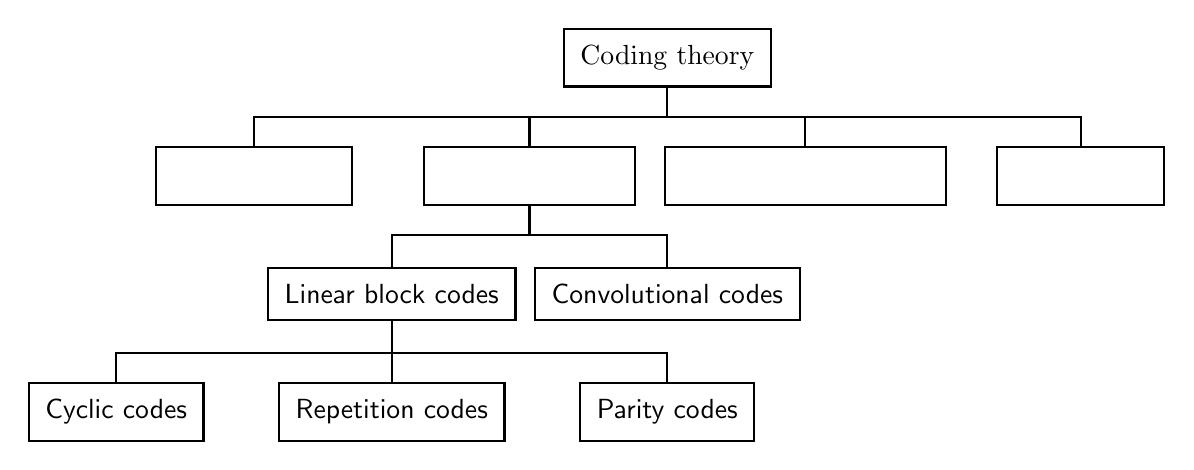
\begin{tikzpicture}[
		-,
		thick,
		every node/.style={
			shape=rectangle,
			inner sep=6pt,
			draw,
			thick,
		},
	]
		\node {Coding theory} [
			edge from parent fork down,
			sibling distance=3.5cm,
		]
			child {
				node[text=white] {\textsf{Source coding}}
			}
			child {
				node[text=white] {\textsf{Channel coding}}
				child { node {\textsf{Linear block codes}}
					child { node {\textsf{Cyclic codes}} }
					child { node {\textsf{Repetition codes}} }
					child { node {\textsf{Parity codes}} }
				}
				child { node {\textsf{Convolutional codes}} }
			}
			child {
				node[text=white] {\textsf{Cryptographic coding}}
			}
			child {
				node[text=white] {\textsf{Line coding}}
			}
		;
	\end{tikzpicture}
\end{document}
